\newpage
\begin{appendices}
\section{Comparisons between Momentum Methods}
\label{appendix:momentum_comp}
The delta rule, at iteration $i+1$, using the gradient descent algorithm with the Classic  heavy-ball Momentum \cite{Polyak1964}, Nesterov \cite{sutskever2013} and Accelerated Nesterov Momentum \cite{nakerst2020gradient} can be summarized in this way:
$$ \Delta^i = \alpha\Delta^{i-1} - \eta\nabla L(w^i +\sigma\Delta^{i-1})$$
$$ w^{i+1} = w^i + \Delta^i$$

When $\sigma = 0$, the delta rule uses the heavy-ball method, and when $\sigma = \alpha$, the Nesterov momentum is used. In \cite{nakerst2020gradient} is shown that can be advantageous to use values of $\sigma$ larger than $\alpha \approx 1$. Instead of using the gradient at an estimated point one step ahead, the gradient is computed at a much further estimated point. This corresponds to an extension of Nesterov and that is why it is called \emph{Accelerated Nesterov Momentum}. Figure \ref{fig:monk1_4_momentum} shows the effect of momentum methods.
\begin{figure}[H]
    \centering
    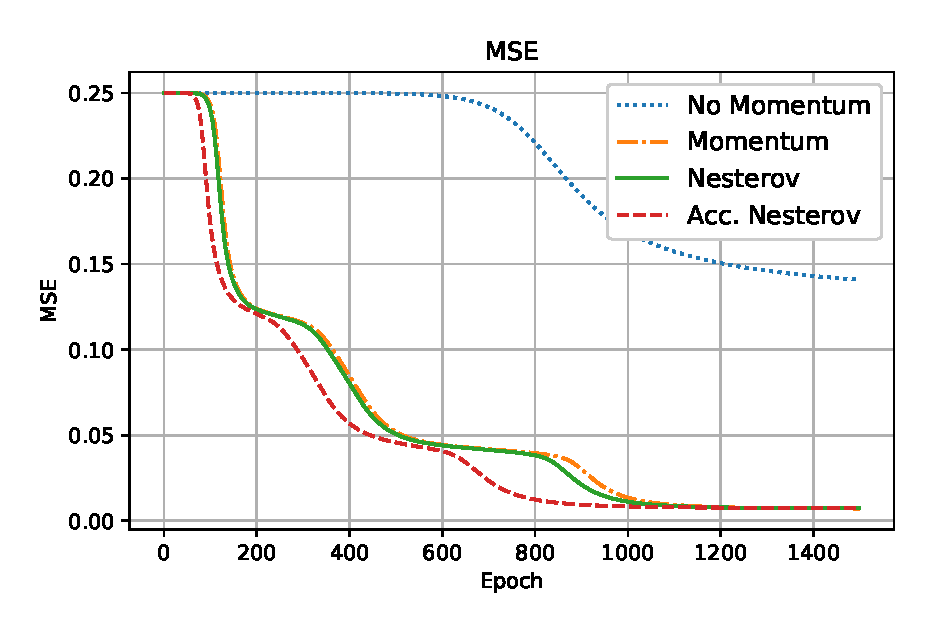
\includegraphics[scale = 0.8]{Images/monk1_4_momentum.eps}
    \caption{Training Learning curves using Monk 1 as dataset with different momentum methods. To compare the learning curves and correctly observe the convergence speed, all the models have been trained starting from the same initial weights.}
    \label{fig:monk1_4_momentum}
\end{figure}
\newpage

\section{Code Examples}
\label{appendix:code_example}
\begin{listing}[!ht]
\inputminted{python}{code/low_api.py}
\caption{A low level API example on the Monk 1 dataset.}
\label{listing:low_api}
\end{listing}

\begin{listing}[!ht]
\inputminted{python}{code/high_api.py}
\caption{A high level API example on the Monk 1 dataset.}
\label{listing:high_api}
\end{listing}

\begin{listing}[!h]
\inputminted{python}{code/model_selection.py}
\caption{Model Selection API example on the CUP dataset.}
\label{listing:model_selection}
\end{listing}

\section{MONKS}
\label{appendix:monks}
\begin{figure}[H]
    \centering
                \begin{subfigure}{0.9\textwidth}
                    \resizebox{\textwidth}{!}{
                        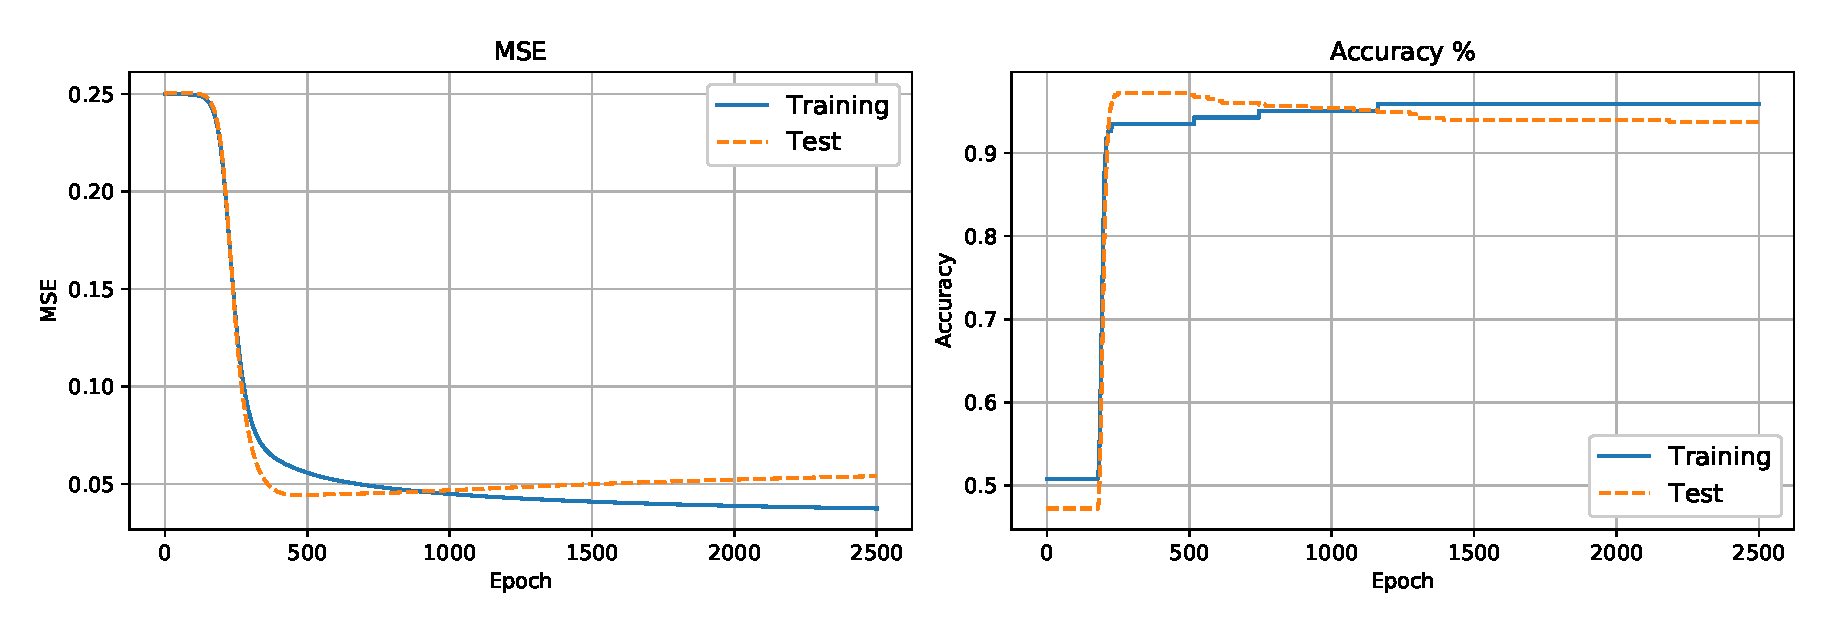
\includegraphics{Images/monks/monk3_overfitting.eps}
                    }
                    \caption{MONK 3 with no regularization}
                    \label{fig:monk3_app}
                \end{subfigure}
                \begin{subfigure}{0.9\textwidth}
                    \resizebox{\textwidth}{!}{
                        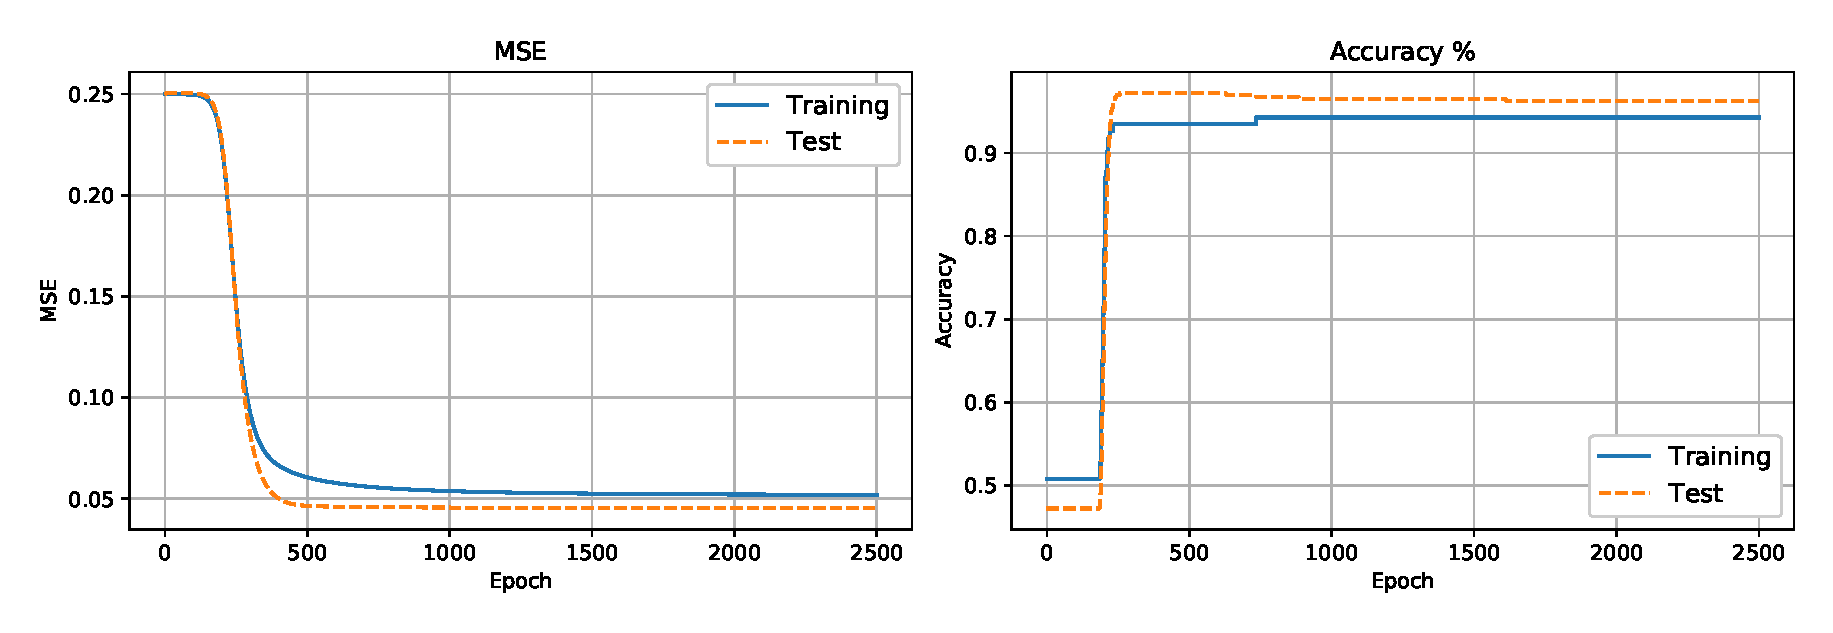
\includegraphics{Images/monks/monk3_over_reg.eps}
                    }
                    \caption{MONK 3 with regularization}
                    \label{fig:monk3_reg_app}
                \end{subfigure}
\caption{Plot of the MSE and accuracy for the MONK 3. In Fig.~\ref{fig:monk3_app}, the model without regularization goes into \emph{overfitting} just before 1000 epochs. Indeed the generalization error measured over the test examples increases, even as the error over the training examples continues to decrease. In Fig.~\ref{fig:monk3_reg_app} is shown how the regularization prevents overfitting.}
\label{fig:monk3_appendix} 
\end{figure}

\begin{table}[h]
\small
    \centering
    \begin{tabular}{ |c|c|c|c|c|c|c|c|c|  }
      \hline
       \textbf{Task} &\textbf{Topology}&\textbf{Batch size}& $\boldsymbol{\eta}$ & $\boldsymbol{\alpha}$ & $\boldsymbol{\lambda}$& \textbf{MSE(TR/TS)} & \textbf{Accuracy(TR/TS)($\boldsymbol{\%}$)}\\
     \hline
    MONK 1 &17$\rightarrow$4$\rightarrow$1 & 1 & 0.4 & 0.8  & 0 & 0.00016 / 0.00023 & 100\% / 100\%\\
    \hline
    MONK 1 &17$\rightarrow$10$\rightarrow$1 & 1 & 0.4 & 0.7  & 0 & 0.00012 / 0.00017 & 100\% / 100\%\\
    \hline
    MONK 1 & 17$\rightarrow$4$\rightarrow$1 & 31 & 0.6 & 0.7  & 0 & 0.00115 / 0.00182 & 100\% / 100\%\\
    \hline
    MONK 2 & 17$\rightarrow$3$\rightarrow$1& 1 & 0.1 & 0.4  & 0 & 0.00205 / 0.00235 & 100\% / 100\%\\
    \hline
    MONK 2 & 17$\rightarrow$10$\rightarrow$1& 1 & 0.1 & 0.4  & 0 & 0.00197 / 0.00229 & 100\% / 100\%\\
    \hline
    MONK 2 & 17$\rightarrow$3$\rightarrow$1& 68 & 0.1 & 0.4  & 0 & 0.00301 / 0.00349 & 100\% / 100\%\\
    \hline
    MONK 2 & 17$\rightarrow$3$\rightarrow$1& 169 & 0.01 & 0.9  & 0 & 0.00970 / 0.01217 & 100\% / 100\%\\
    \hline
    MONK 3 (no reg.)&17$\rightarrow$4$\rightarrow$1 &1 & 0.01 & 0.6  & 0 & 0.04519 / 0.04536 & 95\% / 95\%\\
    \hline
    MONK 3 (no reg.)&17$\rightarrow$10$\rightarrow$1 &1 & 0.01 & 0.5  & 0 & 0.04828 / 0.04398 & 95\% / 95\%\\
    \hline
    MONK 3 (no reg.) & 17$\rightarrow$4$\rightarrow$1&61 &0.6 & 0.3 & 0 & 0.04904 / 0.04483 & 94\% / 96\%\\

     \hline
    \end{tabular}
    \caption{Preliminary cases discovered during the screening phase of the MONKS dataset. Normal momentum was used for online and mini-batch, while Nesterov was used for full batch. Also we used the sigmoid as activation function.}
    \label{tab:monk_screening}
\end{table}

\section{Cup Prepocessing Phase}
\label{appendix:preprop}
During this phase, we analyzed the CUP dataset composed of 20 inputs and 2 targets. From the distributions of the variables (Fig.~\ref{fig:dis}) and correlation matrix (Fig.~\ref{fig:corr_mat}) it can be seen that many variables are strongly correlated to each other: A-I, B-U, C-T, D-P, E-L, F-M, G-S, H-R, N-O and Q-V. Therefore, by eliminating the redundant features (A, B, C, D, E, F, G, H, N, Q), those with correlation equal to 1, it is possible to reduce the dataset to 12 attributes (10 inputs and 2 targets).
\begin{figure}[H]
    \centering
    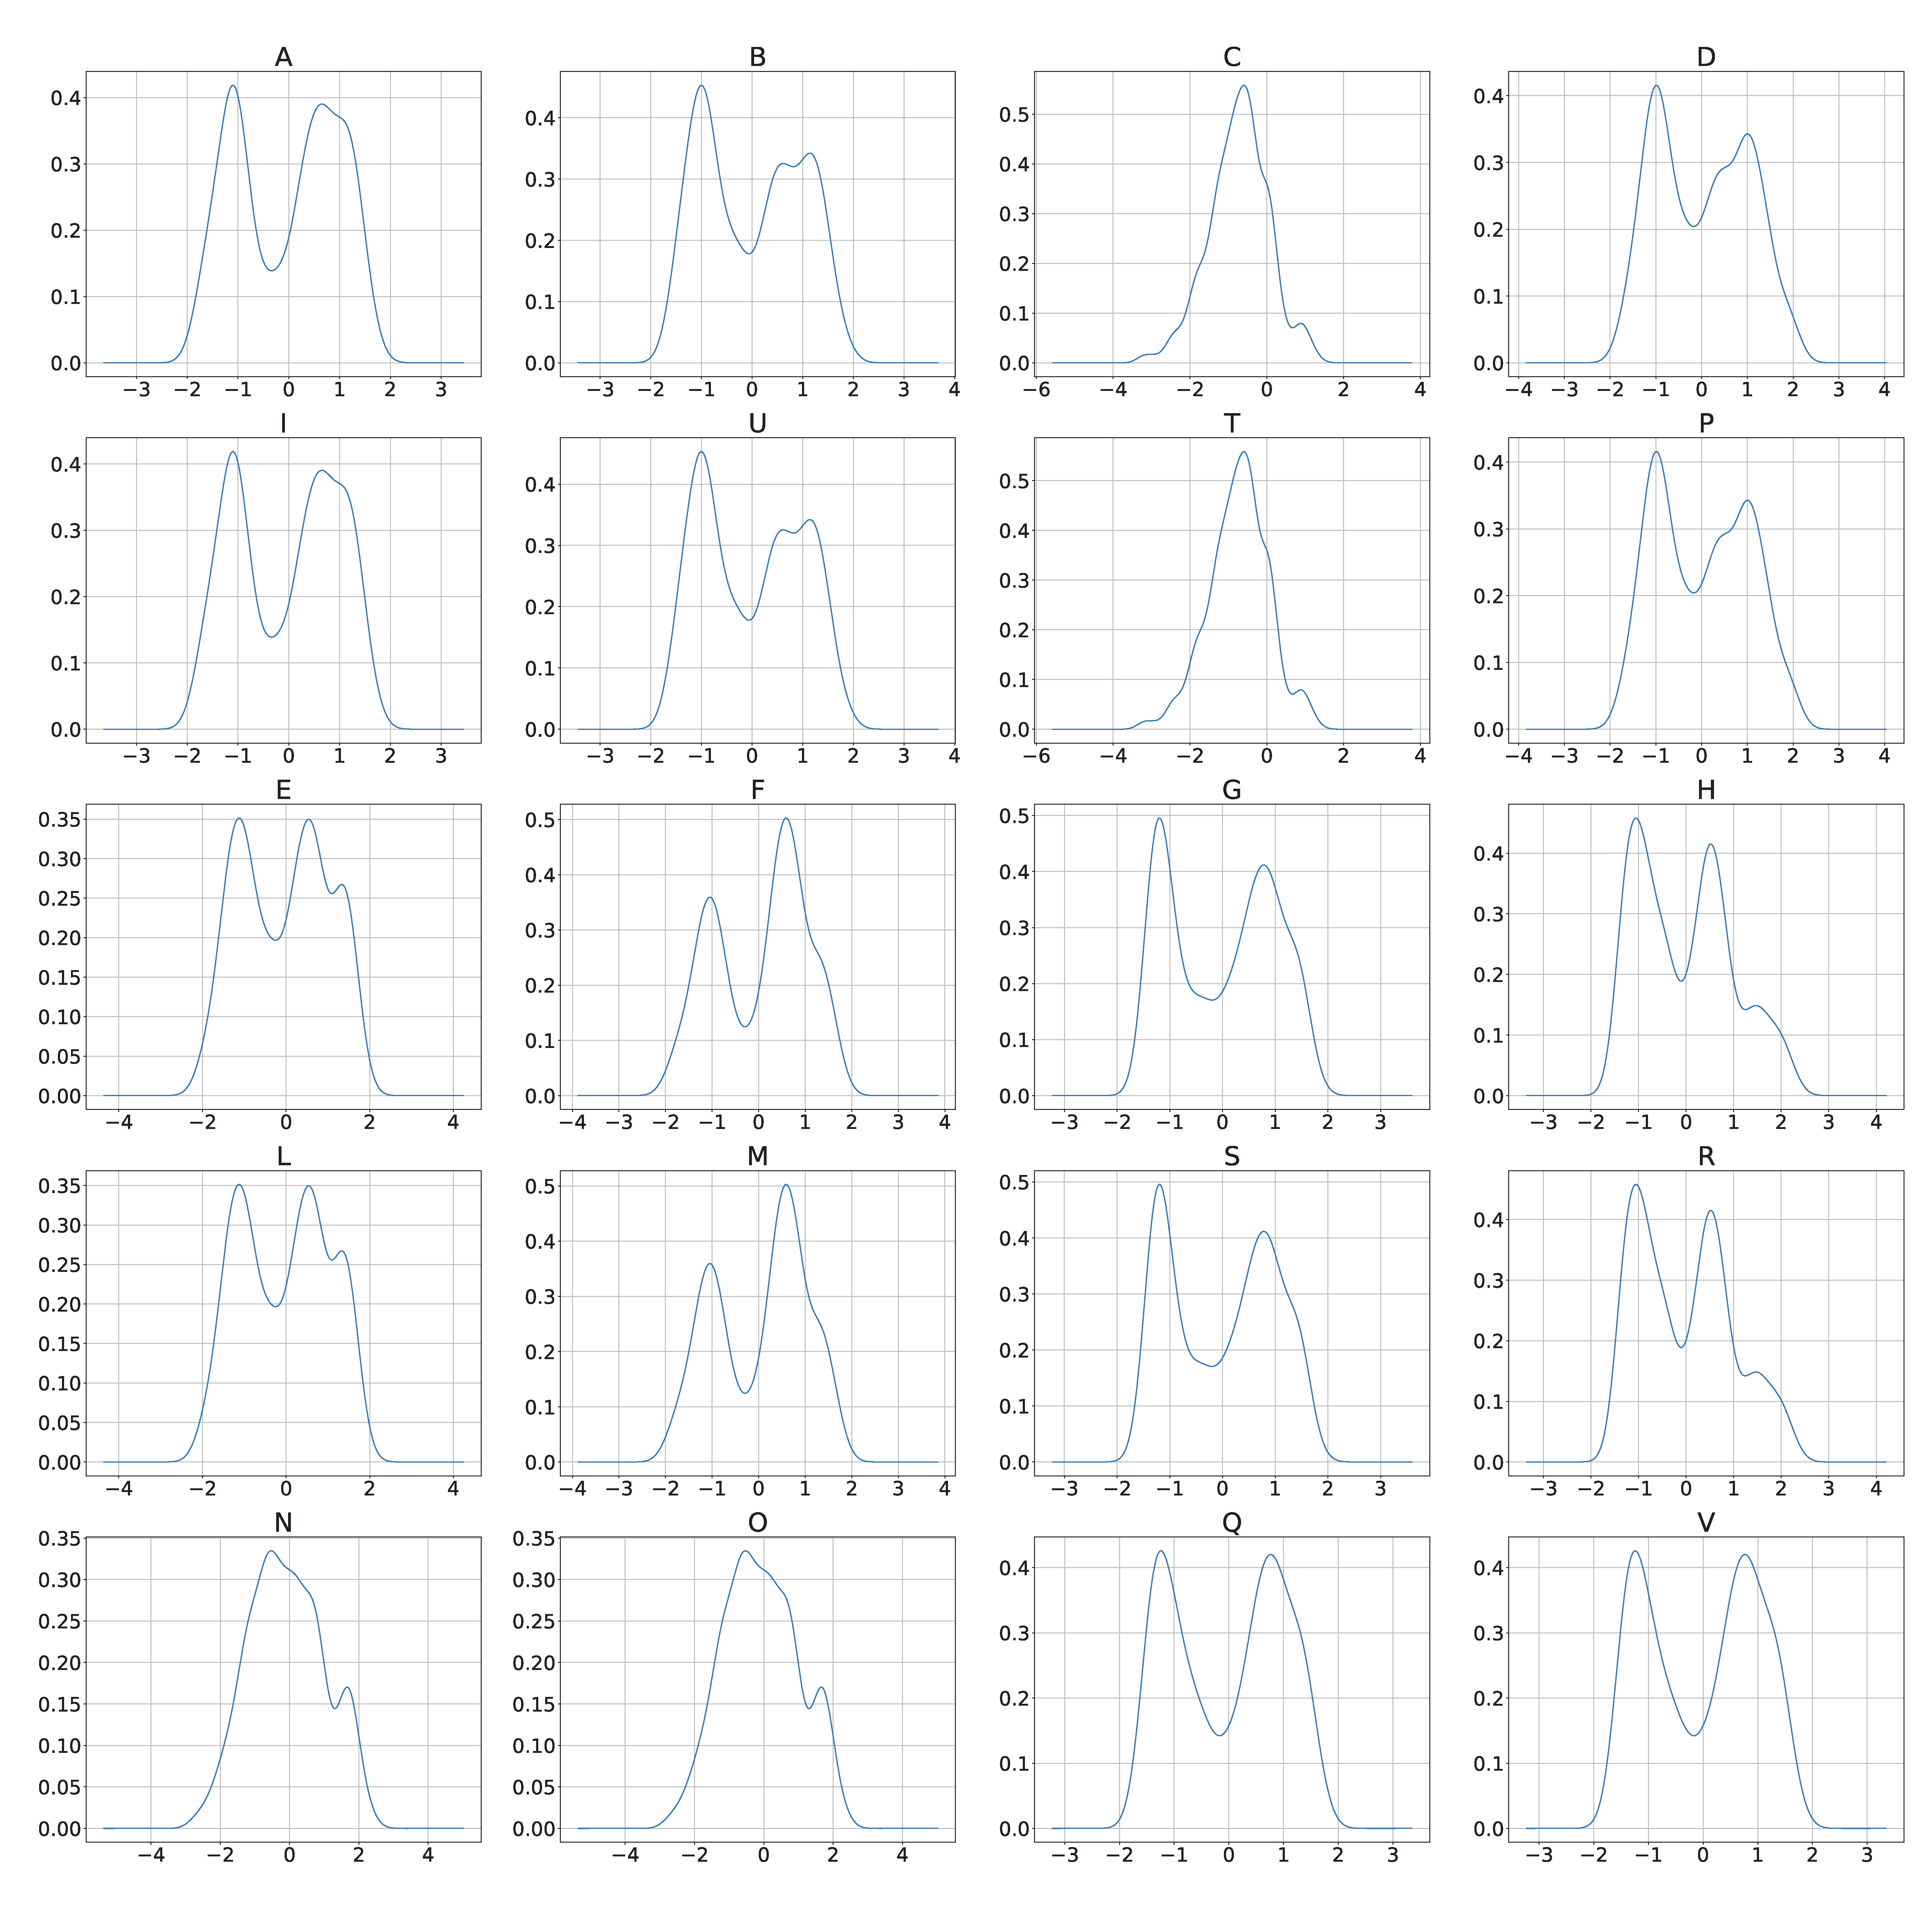
\includegraphics[scale = 0.16]{Images/preprocessing_phase/distributions_2.eps}
    \caption{Distributions of the features, excluded the one representing the id record and those relating to the target.}
    \label{fig:dis}
\end{figure}
\begin{figure}[H]
    \centering
    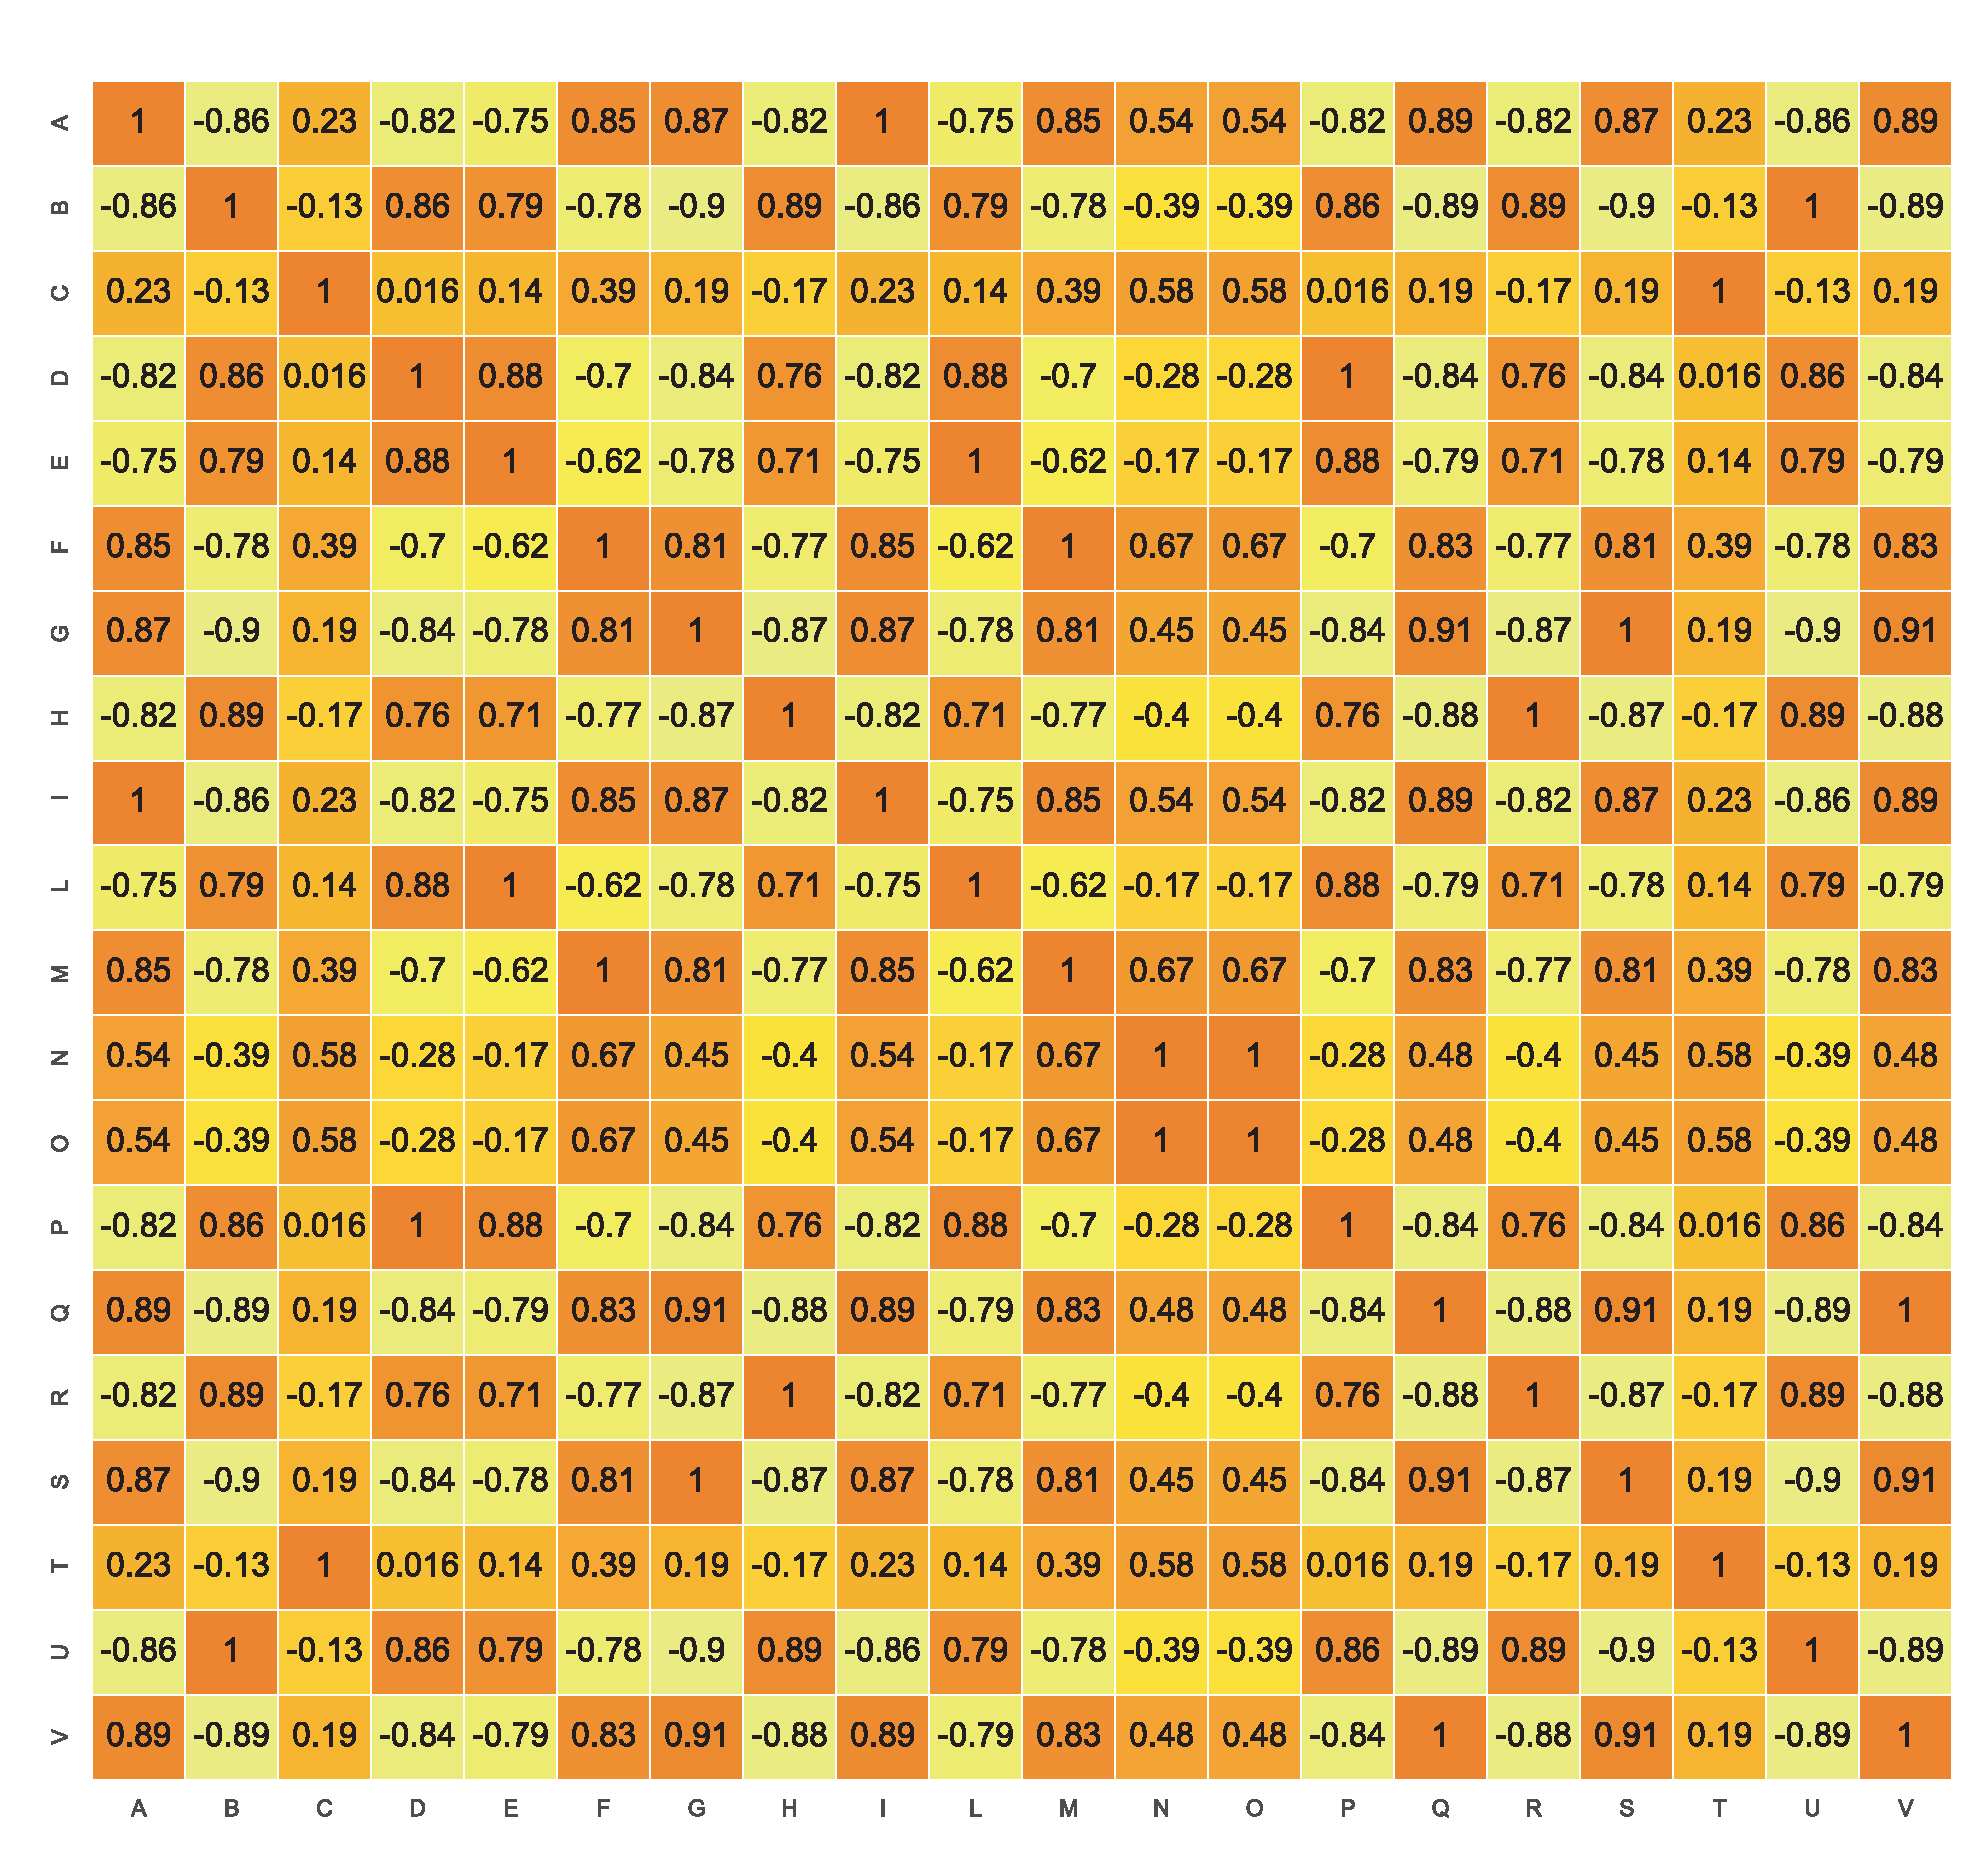
\includegraphics[scale = 0.5]{Images/preprocessing_phase/correlation_matrix_2.eps}
    \caption{Correlation matrix.}
    \label{fig:corr_mat}
\end{figure}
\end{appendices}
